

\begin{center}
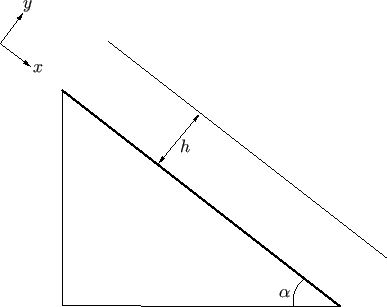
\includegraphics[width=4cm]{python_codes/fieldstone_59/images/setup}\\
{\captionfont REDO with tikz}
\end{center}

\paragraph{Linear viscous fluid}

We start from the Stokes equation for isoviscous fluids:
\[
\eta \Delta \vec{\upnu} - \vec\nabla p + \rho \vec{g} = \vec{\bm 0}
\]
Assuming that the fluid is incompressible and that the incline is infinite, 
then $\vec{\upnu}=(u(y),0)$.
The $x$-component of the equation then writes:
\[
\eta(\frac{\partial^2 u}{\partial x^2}+\frac{\partial^2 u}{\partial y^2} )
- \frac{\partial p}{\partial x} + \rho g_x =0
\]
\[
\Rightarrow 
\eta\frac{\partial^2 u}{\partial y^2} 
+ \rho g \sin\alpha =0
\]
since $\partial_x\rightarrow 0$.
This 2nd order ODE can be integrated twice. The two integration constants are 
determined by setting $u(y=0)=0$ and the shear stress to be zero at the (free)
surface. The velocity profile is given by:
\[
u(y)=\frac{\rho g \sin \alpha}{2 \eta} (2h-y)y
\]
Also, we have 
\[
\dot{\varepsilon}_{xx}=0
\qquad
\dot{\varepsilon}_{yy}=0
\qquad
\dot{\varepsilon}_{xy}
=\frac{1}{2}( \frac{\partial u}{\partial y} + \frac{\partial v}{\partial x} )
=\frac{1}{2} \frac{\partial u}{\partial y} 
= \frac{\rho g \sin \alpha}{2 \eta} (h-y)
\]

For $\alpha\sim 0.5-1$\degree, then $\sin\alpha\sim 0.01$. 
We also have $\rho\sim1000$, $g\sim$10, $\eta\sim 10^m$, $h\sim2500$.
The velocity is maximum at the surface and is given by
\[
u(y=h)=
\frac{\rho g \sin \alpha}{2 \eta}h^2 
\sim \frac{1000 \cdot 10 \cdot 0.01}{ 2\cdot 10^m}2500^2
\sim 3\cdot 10^{8-m}
\]



\begin{center}
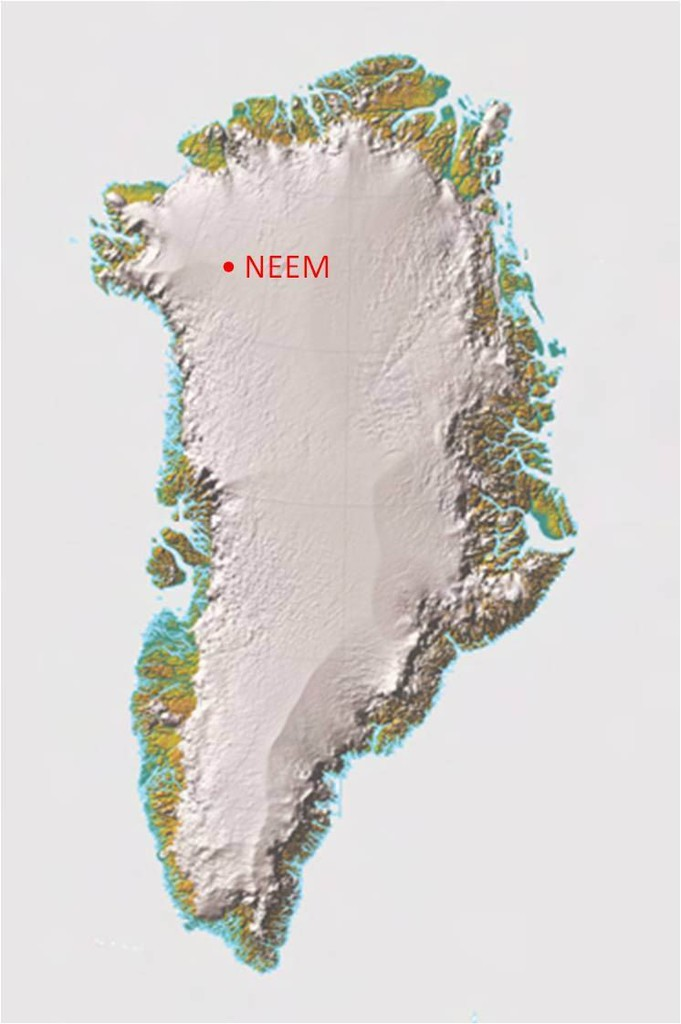
\includegraphics[width=6.4cm]{python_codes/fieldstone_59/images/neem}
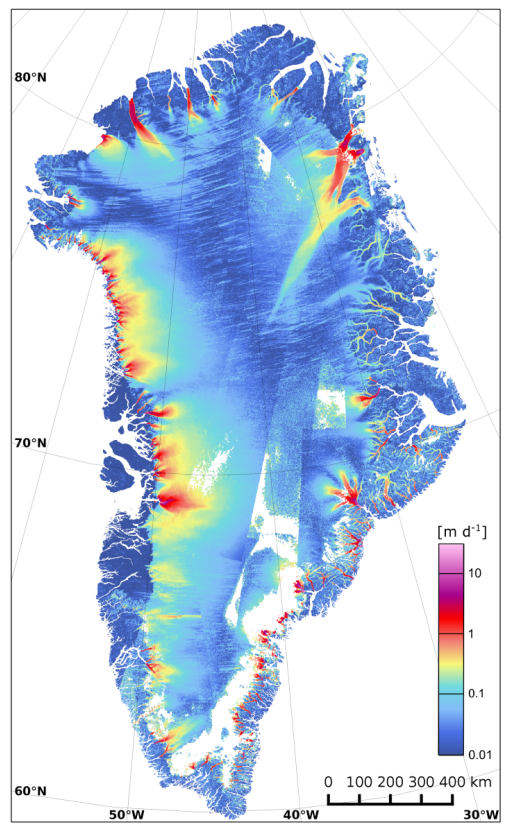
\includegraphics[width=6cm]{python_codes/fieldstone_59/images/narh15}\\
{\captionfont Ice velocity map (magnitude, in logarithmic scale) of the Greenland Ice Sheet
derived from SAR data of the Sentinel-1A satellite, acquired in Interferometric Wide Swath
Mode (IW) between January and March 2015. Taken from \cite{narh15}.}
\end{center}
As shown on the figures above the typical ice sheet velocity values around the NEEM ice core 
is $\sim 0.03m/day \simeq 3\cdot 10^{-7}$m/s. 
Then in order for the top of the ice sheet to flow at this speed we require $m=15$.

Having obtained the (effective linear) viscosity of the ice, i.e. $\eta\simeq 10^{15}$Pa.s,
we can compute the strain rate at the bottom and in the middle:
\[
\dot{\varepsilon}_{xy}(y=0) 
= \frac{\rho g \sin \alpha}{2 \eta} h
\sim \frac{1000\cdot 10 \cdot 0.01}{2 \cdot 10^{15}}2500
\sim 10^{-10}\text{s}^{-1}
\]
\[
\dot{\varepsilon}_{xy}(y=h/2) 
= \frac{\rho g \sin \alpha}{2 \eta} \frac{h}{2}
\sim \frac{1000\cdot 10 \cdot 0.01}{2 \cdot 10^{15}}2500
\sim 5\cdot 10^{-11}\text{s}^{-1}
\]
which are reasonable values as confirmed by the following figure (yellow line):  
\begin{center}
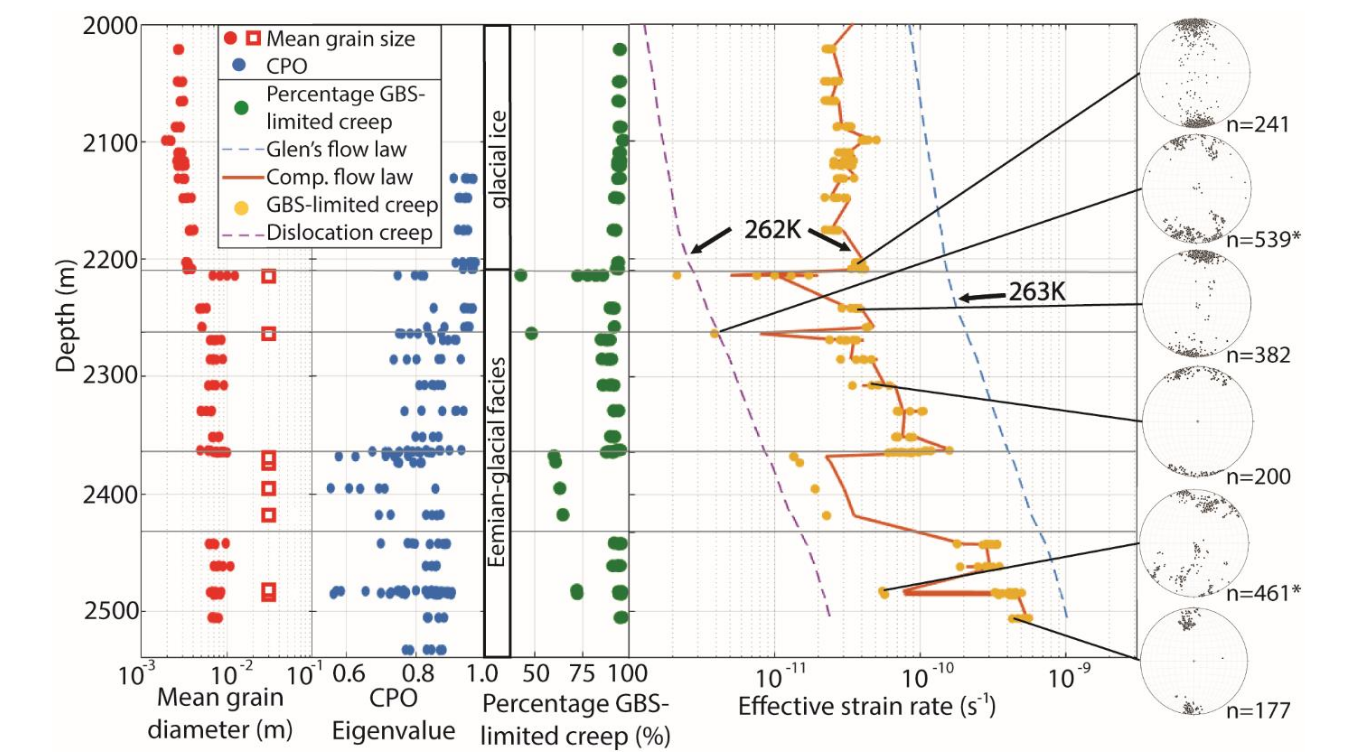
\includegraphics[width=11cm]{python_codes/fieldstone_59/images/kudd19}\\
{\captionfont Taken from Kuiper et al \cite{kudd19}.}
\end{center}

The conclusion from this exercise is that {\sl if} ice could be described by 
a linear viscous fluid flowing on an infinite incline, a viscosity of $\eta\simeq 10^{15}$Pa.s
would yield observations that match recorded velocities and strain rates. 

However, the picture is way more complex, as it was observed very early on 
by Glen in 1955 \cite{glen55} and many others later. It was then found that 
\[
\dot{\varepsilon} = A \tau^n,
\]
i.e. the ice behaves as a power-law fluid \ref{sec:XXXX}, with 
$n=3$ and $A\simeq 2.4\cdot 10^{-24}$ at 0\degree.

More recently Kuiper et al. \cite{kuwd19,kudd19} derived a composite flow law 
to model deformation in the NEEM deep ice core. 
They start from the flow law proposed by Goldsby \& Kohlstedt \cite{goko01}:
\[
\dot{\varepsilon}_T = \dot{\varepsilon}_{disl} + 
\left(\frac{1}{ \dot{\varepsilon}_{basal}} + \frac{1}{ \dot{\varepsilon}_{GBS}} \right)^{-1} 
+  \dot{\varepsilon}_{diff}
\]
where $\dot{\varepsilon}_T$  is the total strain rate, 
composed of strain rates for basal slip accommodated by non-basal slip or dislocation creep,
$\dot{\varepsilon}_{disl}$ , grain boundary sliding (GBS) accommodated by basal slip, 
$\dot{\varepsilon}_{basal}$ , and basal slip accommodated by GBS, 
$\dot{\varepsilon}_{GBS}$ , and diffusion creep, 
$\dot{\varepsilon}_{diff}$. Each of these creep mechanisms can be described by a 
power law relation of the form:
\[
\dot{\varepsilon} = A \tau^n d^{-p} \exp \left( -\frac{Q+pV}{RT} \right)
\]
where $A$ is a material parameter, $\tau$ is the differential stress (MPa), 
$n$ is the stress exponent, $d$ is the grain size diameter (m), 
$p$ is the grain size exponent, $Q$ is the activation energy for the creep 
mechanism at stake (J$\cdot$mol$^{-1}$ ), $p$ is the hydrostatic pressure (MPa), 
$V$ the activation volume (m$^3$ mol$^{-1}$), 
$R$ is the gas constant (J K$^{−1}$ mol$^{-1}$ ), and $T$ the absolute temperature (K). 
The effect of $pV$ is assumed to be very small (Durham and Stern, 2001) \cite{dust01} 
and is ignored for the remainder of this work.

As explained in \cite{kuwd19} the composite flow law can actually be simplified to:
\[
\dot{\varepsilon}_T = \dot{\varepsilon}_{disl} + \dot{\varepsilon}_{GBS}
\]
The material parameters for these deformation mechanisms are available in \cite{kudd19}:
\begin{center}
\begin{tabular}{lcccc}
\hline
Creep regime & A & n & p & Q (J$\cdot$mol$^{-1}$) \\
\hline\hline
Glen's flow law ($T<263$K) &$3.61\cdot10^5$ MPa -3.0 s −1 &3.0 &0 &60\\
Glen's flow law ($T>263$K) &$1.73\cdot10^{21}$ MPa -3.0 s −1 &3.0 &0 &139\\
\hline
Dislocation creep ($T<262$K) & $5.0\cdot10^5$ MPa -4.0 s −1 &4.0 &0 &64\\
Dislocation creep ($T>262$K) &$6.96\cdot 10^{23}$ MPa -4.0 s −1 &4.0 &0 &155\\
\hline
GBS-limited creep ($T<262$K) & $1.1\cdot 10^2$ MPa$^{-1.8}$ m$^{1.4}$ -1 &1.8 &1.4 &70\\
GBS-limited creep ($T>262$K) & $8.5\cdot10^37$ MPa$^{-1.8}$ m$^{1.4}$ s −1 &1.8 &1.4 &250\\
\hline
\end{tabular}
\end{center}



